%!TEX TS-program = xelatex
%!TEX encoding = UTF-8 Unicode

\documentclass[11pt,tikz,border=1]{standalone}
\usepackage{pgfplots}
\usetikzlibrary{positioning}

\begin{document}
  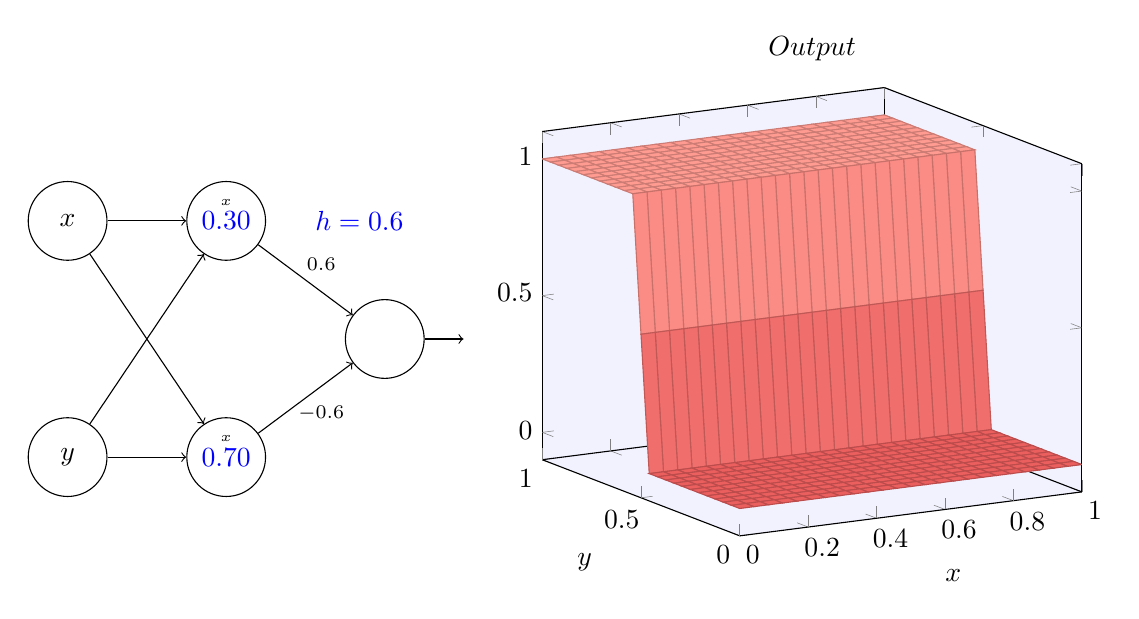
\begin{tikzpicture}[
    neuron/.style={circle,draw,inner sep=0pt,minimum size=10mm}
    ]
    
    \begin{scope}
      \node(n) [neuron] {};
      
      \node(h0) [neuron,left=of n,yshift=1.5cm] {};
      \node(h1) [neuron,left=of n,yshift=-1.5cm] {};
      
      \node(x) [neuron,left=of h0] {$x$};
      \node(y) [neuron,left=of h1] {$y$};
    
      \draw[->] (x) to (h0);
      \draw[->] (x) to (h1);
      \draw[->] (y) to (h0);
      \draw[->] (y) to (h1);
  
      \node (s0) [blue] at (h0.center) {$0.30$};
      \node at (s0.north) {\tiny $x$};
      \node (s1) [blue] at (h1.center) {$0.70$};
      \node at (s1.north) {\tiny $x$};
      
      \node [blue,right=5mm of h0] {$h = 0.6$};

      \draw[->] (h0) -- node [xshift=2mm,yshift=2mm] {\scriptsize $0.6$} (n);
      \draw[->] (h1) -- node [xshift=2mm,yshift=-2mm] {\scriptsize $-0.6$} (n);
      
      \draw[->] (n) -- ++(1cm, 0);
    \end{scope}
    
    \begin{scope}[xshift=2cm,yshift=-2.5cm]    
      % FIXME: rotate the zlabel, change plot color, and move z axis to right
      \begin{axis}[
        view={-30}{15},        
        axis background/.style={fill=blue!5},
        xlabel=$x$,
        ylabel=$y$,
        title=$Output$,
        colormap={simple}{rgb255=(235,95,95) rgb255=(255,155,145)},
        declare function={
          sigmaInverse(\z)=ln(\z/(1-\z));
          f(\x)=0.2+0.4*\x*\x+0.3*\x*sin(15*deg(\x))+0.05*cos(50*deg(\x));
        }]
        \addplot3[surf,domain=0:1] {
          1 / (1 + exp(-(1000) * y - (-0.5 * 1000)))
        };
      \end{axis}
    \end{scope}
    
  \end{tikzpicture} 
\end{document}
